In this section, we present a method for extracting behavioural~\emph{scenarios} from
system control programs and synthesising them into application-specific
integrated circuits implementing execution of these scenarios. We exploit the
existing formalism of Conditional Partial Order Graphs (CPOGs)~\cite{CPOG} for
synthesising scenarios. CPOGs are included~\cite{scenco-tool} as a plugin in
the~\textsc{Workcraft} framework~\cite{workcraft-tool}, which implements
the scenario specification and synthesis methods and handles the mapping of
CPOGs into interconnection of logic gates to produce a physical implementation
of the system microcontroller.

\subsection{Extracting scenarios from programs}

We defined a \textit{scenario} to be a list of
instructions that are executed in a specified order. Formally, a scenario
$s=(\mathcal{I},\prec)$ is a \textit{partial order}~(PO)~\cite{PO},
i.e. a binary precedence relation $\prec$ defined on a set of instructions
$\mathcal{I}$ that satisfies two properties:

\begin{itemize}
    \item Irreflexivity: $\forall a \in \mathcal{I}, \neg(a \prec a)$
    \vspace{+1mm}
    \item Transitivity: $\forall a, b, c \in \mathcal{I}, (a \prec b) \wedge (b
    \prec c) \Rightarrow (a \prec c)$
\end{itemize}

To mine scenarios from programs, we partially reuse the methodology
used for construction of the concurrency oracles from the previous section.
The methodology is implemented with the following procedure:

\subsubsection{Scenario extraction:}
\begin{enumerate}
    \item Calculate the static data dependencies of the program.
    \item Construct the static dependencies graph.
    \item Remove the data-vertices preserving the transitive connections between
        instruction-vertices.
    \item A~\emph{transitive closure} of the resulting graph will display the
        partial order on the set of events represented as instruction-vertices.
\end{enumerate}

\subsection{Scenario encoding and synthesis}

In the context of this paper, we consider control systems which are programmed
in low-level assembly-like languages. Using the procedure from the previous subsection,
we can extract behavioural scenarios, represented as partial orders, from the
system's control programs. It is often the case for these partial orders to have
some functionality shared. The existing Conditional Partial Order Graphs
formalism allows compositional combination of multiple partial orders into one
structure, leading for more efficient implementation of the composed
specification, in comparison to one implementing the scenarios separately.

\subsubsection{Program synthesis:}
\begin{enumerate}
    \item Extract all scenarios from the set of system's control programs.
    \item Synthesis the scenarios into a CPOG to enable functionality sharing.
    \item Use the CPOG model workflow (optimisation, compilation to hardware circuit).
\end{enumerate}

The Conditional Partial Order Graphs formalism is supported in the open source
framework WORKCRAFT, which facilitates construction and visualisation of partial
orders, their synthesis into a CPOG and compilation to logical circuits.

In the next subsection, we will illustrate the scenario instruction and
synthesis procedures on a simple example. We will consider a system and two
control programs, extract the scenarios from these programs and synthesise them
into a CPOG with some functionality shared.

\subsection{Example}

To illustrate the use of the scenario extraction procedure, let us sketch an
example of system controlling an hypothetical dual-motor autonomous vehicle.
The vehicle has two motors directly driving its left and right front wheels.
The system control unit has a simple application-specific instruction set, 4
general-purpose registers and a memory unit with 255 cells. The velocity of the
left and right motor is controlled by the values in the cell 0 and 1, respectively.
The motor's velocity may be adjusted with the command~\hs{Adjust}
supplying the value in a register and referring the motor index (0 or 1).

The first program (figure~\ref{fig-scenarios-drive-straight}, on the left) implements
the ``drive straight'' behaviour, driving both wheels with the same power.
The graph on the right pictures the extracted partial order.

\begin{figure}
\vspace{-5mm}
\centering
  \begin{minipage}[b]{0.5\textwidth}
\begin{minted}[linenos]{haskell}
Load R0 254
Adjust R0 0
Adjust R0 1
\end{minted}
\vspace{5mm}
\end{minipage}
% \hfill
\begin{minipage}[b]{0.4\textwidth}
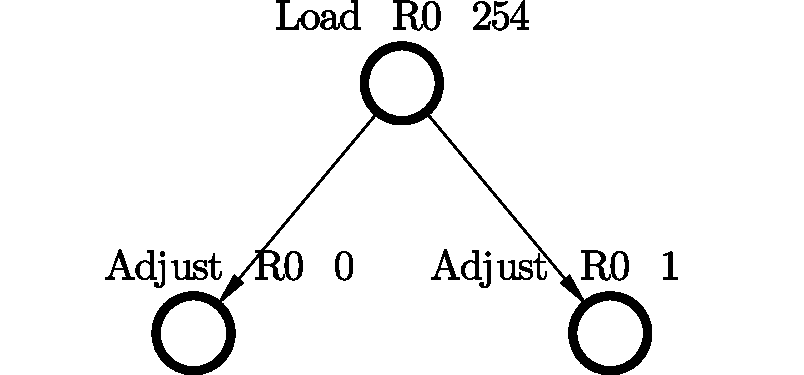
\includegraphics[scale=0.35]{img/ataed-scenario-drive-straight.pdf}
\end{minipage}
\caption{Simple behaviour scenario and the corresponding
partial order.\label{fig-scenarios-drive-straight}}
\end{figure}

Another behaviour is ``drive and turn'' is implemented by adjusting the velocities
with different values (figure~\ref{fig-scenarios-turn}). In this case, the
resulting partial order contains two independent components.

\begin{figure}
\vspace{-5mm}
\centering
  \begin{minipage}[b]{0.5\textwidth}
\begin{minted}[linenos]{haskell}
Load R0 254
Load R1 255
Adjust R0 0
Adjust R1 1
\end{minted}
\vspace{5mm}
\end{minipage}
% \hfill
\begin{minipage}[b]{0.4\textwidth}
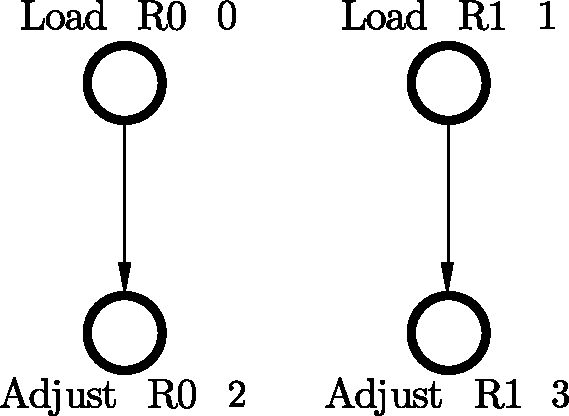
\includegraphics[scale=0.35]{img/ataed-scenario-turn.pdf}
\end{minipage}
\caption{Simple behaviour scenario and the corresponding
partial order.\label{fig-scenarios-turn}}
\end{figure}

The figure~\ref{fig-scenarios-composition} displays the Conditional Partial Order Graph
which represents the composition of the two behaviours. On of the partial orders
extracted from the second program gets merged into the one extracted from the first
program, thus rendering the CPOG composition to be more compact then simple overlay of
the extracted scenarios.

\begin{figure}
\centerline{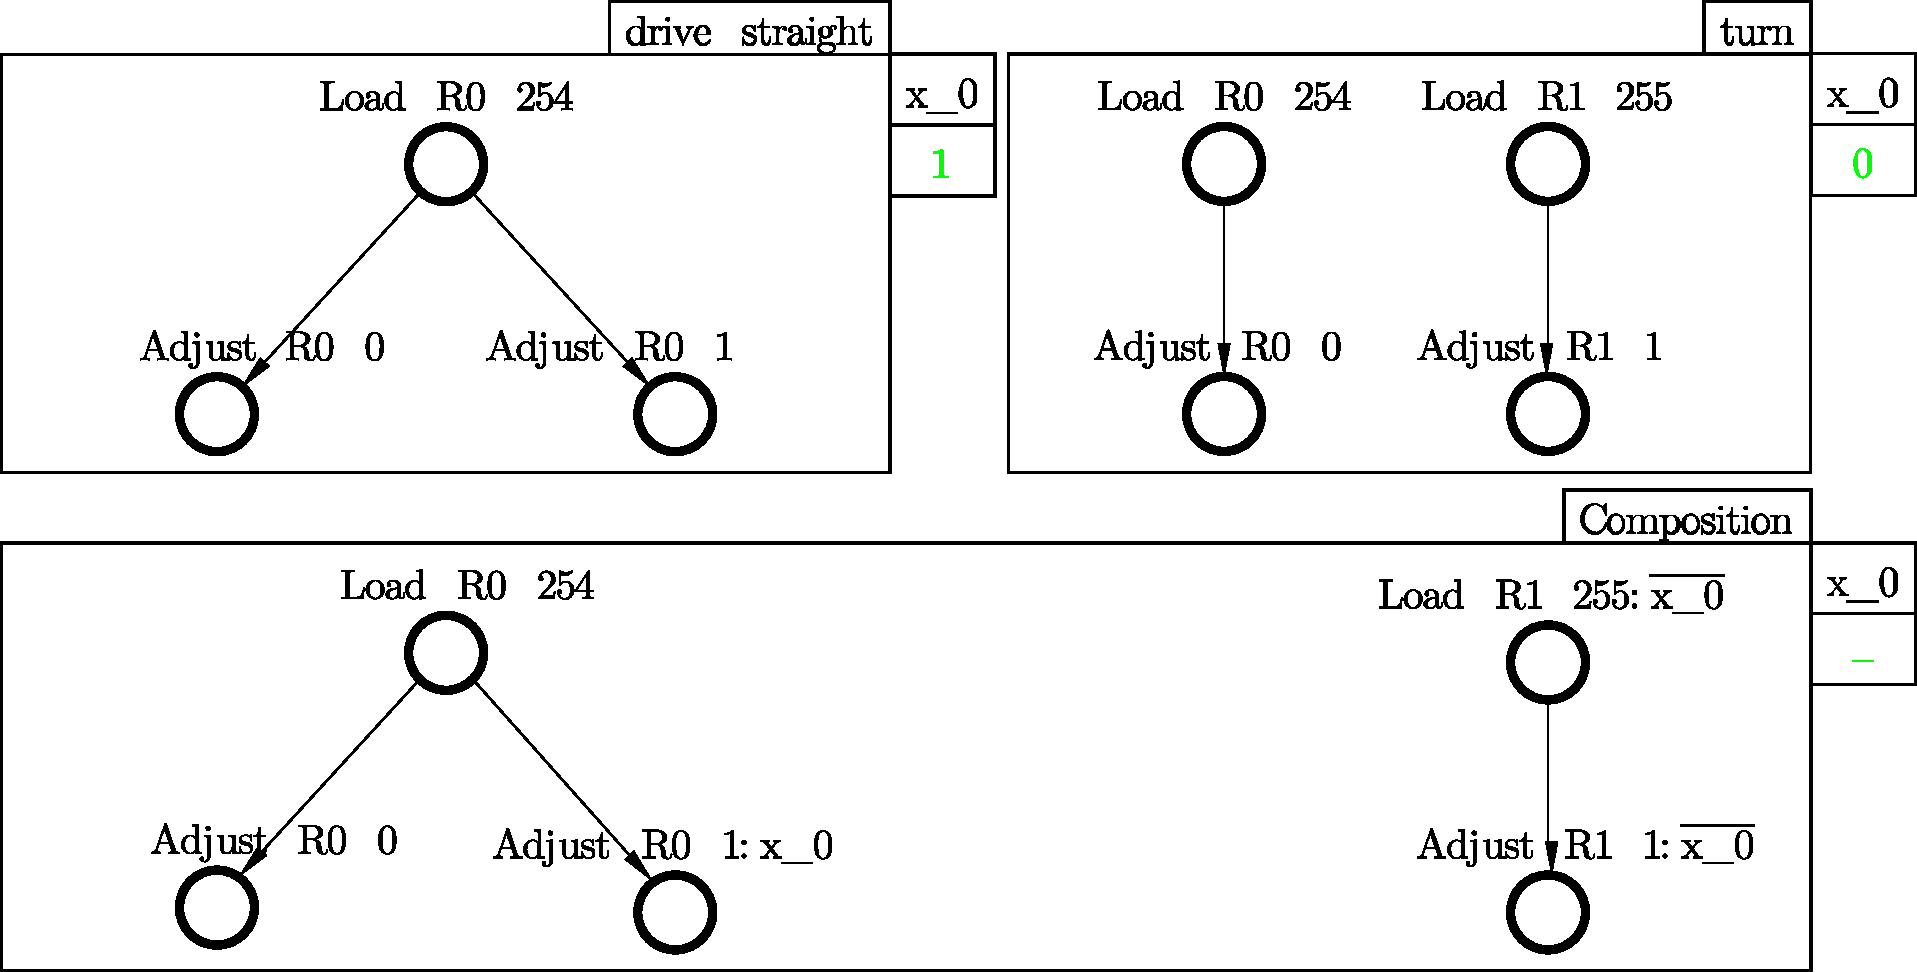
\includegraphics[scale=0.35]{img/ataed-composition.pdf}}
\caption{Two operation scenarios and their composition.\label{fig-scenarios-composition}}
\end{figure}

